\subsection{Security}
This subsection is intended to give a description on how the system should be developed to ensure security against accidental or malicious accesses, unauthorized uses or modifications of the system itself.
myTaxiService is a Three-Tier architecture and the Application Side should be considered as the Presentation Tier, the Server Side instead, contains the Logic Tier and the Data Tier.

	\subsubsection{Application and User Interface Side}
	Here is implemented the Presentation Tier of the system.
	On the application side should be implemented a first security check on the credentials that the user has to insert. In particular: 
		\begin{itemize}
			\item Passwords must be at least 8 characters long and must contain digits and alphabetic characters.
			\item The emails must match the regular expression:\\ \textquotedblleft\textasciicircum\textbackslash w+@\lbrack a-zA-Z\_\rbrack\plus?\textbackslash.\lbrack a-zA-Z\rbrack\{2,3\}\$".
		\end{itemize}  
	These controls are made in real time by the application to give a better user's experience avoiding the reload of the application pages, others checks are delegated to the server side to avoid users to exploit the security system.
	If the user's data are not valid for this layer, then the application should not call for server functions.
	To call remote functions, the system must implement HTTP-POST requests instead of HTTP-GET requests.

	\subsubsection{Server Side}
	The server side is divided in two tiers: Logic Tier and Data Tier.
	\\
	Logic tier is the one that receives application requests and queries the data tier. In this tier are implemented all the checks about the user credentials that have been sent by the application side. In particular:
		\begin{itemize}
			\item In the registration procedure, the username and the email must not be already registered into the database; passwords are encrypted with MD5 hashing;
			\item In the login procedure, the username must be registered and the related password must be equal to the given one to give a positive reply.
		\end{itemize}
	~\\
	Data tier is the one that memorizes all the system's data and makes them available to the logic tier (DBMS).
	~\\
	To improve the security of our system, the server side is divided in two servers:
		\begin{itemize}
			\item Web Server, that contains the web application and the server application.
			\item Database Server, that contains the interface to the database.
		\end{itemize}

	\begin{figure}[H]
		\centering
		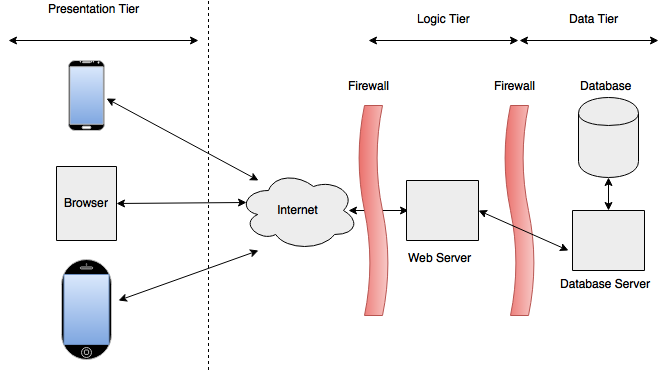
\includegraphics[width=\textwidth, scale=0.5]{IMG/ServerArchitecture.png}
		\caption{Server Architecture}\label{sec:FigureServerArchitecture}
	\end{figure}